\documentclass[10pt]{article}

% Packages
\usepackage{caption}
\usepackage{graphicx}
\usepackage[bf,small]{titlesec}
\usepackage{float}
\usepackage{hyperref}
\usepackage{subcaption}

\restylefloat{figure}

\begin{document}

\section*{Graf's addition theorem}

\begin{figure}[H]
\centering
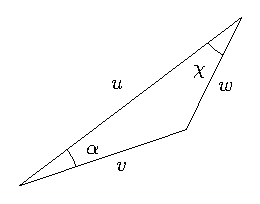
\includegraphics{media/graf.eps}
\caption{Graf's addition theorem}
\end{figure}

\emph{Graf's addition theorem} says
%
\[ C_\nu(w) e^{i \nu \chi} = \sum_{k = -\infty}^{\infty} C_{\nu + k}(u) \;
J_k(v) e^{i k \alpha} \]
%
where $C_\nu$ can be a Hankel or Bessel function of index $\nu$. This holds when
$|u| > |v|$. \footnote{See for instance \url{http://dlmf.nist.gov/10.23\#ii}}

\section*{Expansions}

In all subsequent formulas, $\theta_{xy}$ refers to the angle of the vector
$x-y$ above the horizontal.

\begin{figure}[H]
\centering
\begin{subfigure}[b]{0.4\linewidth}
\centering
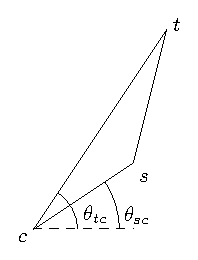
\includegraphics{media/m-expn.eps}
\caption{Multipole expansion}
\end{subfigure}
%
\hspace{1cm}
%
\begin{subfigure}[b]{0.4\linewidth}
\centering
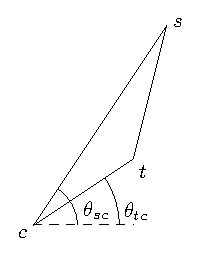
\includegraphics{media/l-expn.eps}
\caption{Local expansion}
\end{subfigure}

\caption{Multipole and local expansions}

\end{figure}

For a multipole expansion, we wish to evaluate $H_0^1(|t - s|)$ where the target
is farther from the center than the source. The multipole expansion takes the
form
%
\[ H_0^{(1)}(|t - s|) = \sum_{k = -\infty}^{\infty} \underbrace{J_k(|s - c|)
  e^{- i k \theta_{sc}}}_{\textrm{coefficients}} H_k^{(1)}(|t - c|) e^{i k
  \theta_{tc}}. \]
%
In the local expansion, the target is closer to the center than the source. The
local expansion takes the form
%
\[ H_0^{(1)}(|t - s|) = \sum_{k = -\infty}^{\infty} \underbrace{H_k^{(1)}(|s -
  c|) e^{i k \theta_{sc}}}_{\textrm{coefficients}} J_k(|t - c|) e^{- i k
  \theta_{tc}}. \]

\section*{Multipole-to-multipole and local-to-local translations}

We wish to shift the center of the expansion $c_1$ to a new center $c_2$
satisfying $|c_1 - c_2| < |s - c_1|$. The goal is to derive a formula for the
new coefficients based on the old coefficients and $c_1 - c_2$. This can be done
with the help of Graf's addition theorem.

\begin{figure}[H]
\centering
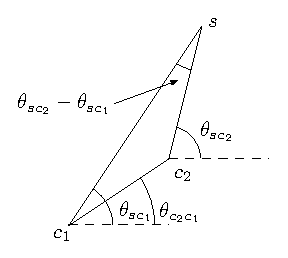
\includegraphics{media/m2m-l2l-translation.eps}
\caption{Multipole-to-multipole and local-to-local translation}
\end{figure}
For shifting the multipole coefficients:
\[ J_k(|s - c_2|) e^{-i k \theta_{sc_2}} = \sum_{l = -\infty}^{\infty}
\underbrace{J_{k + l}(|s - c_1|) e^{-i (k + l) \theta_{sc_1}}}_{\textrm{old
    coefficients}} \; J_l(|c_2 - c_1|) e^{i l \theta_{c_2 c_1}}. \]
%
In a similar way, for shifting the local expansion coefficients:
%
\[ H_k^{(1)}(|s - c_2|)e^{ik\theta_{sc_2}} = \sum_{l = -\infty}^{\infty}
\underbrace{H_{k + l}^{(1)}(|s - c_1|) e^{i(k + l) \theta_{sc_1}} }_{\textrm{old
    coefficients}} \; J_l(|c_2 - c_1|) e^{-i l \theta_{c_2 c_1}}. \]


\section*{Multipole-to-local translation}

Given a multipole expansion with center $c_1$, we wish to shift to center $c_2$
where $c_1$ and $c_2$ satisfy $|c_2 - c_1| > |s - c_1|$. Furthermore, the
coefficients at the new center will be coefficients for a local expansion.

\begin{figure}[H]
\centering
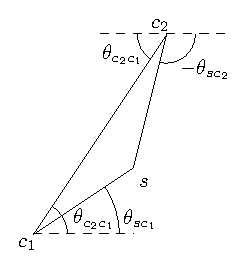
\includegraphics{media/m2l-translation.eps}
\caption{Multipole-to-local translation}
\end{figure}

The translated coefficients satisfy
%
\[ H_k^{(1)}(|s - c_2|) e^{i k \theta_{sc_2}} = (-1)^k \sum_{l = -\infty}^{\infty}
\underbrace{J_l(|s - c_1|) e^{- i l \theta_{sc_1}}}_{\textrm{old coefficients}}
H_{k + l}^{(1)}(|c_1 - c_2|) e^{i(k + l)\theta_{c_2c_1}}. \]

\end{document}
